\documentclass[11pt, openright]{report}
\makeatletter\@twosidetrue\makeatother
\usepackage{setup}


\makeatletter
\newcommand\frontmatter{%
    \cleardoublepage
    \setcounter{secnumdepth}{0}
  %\@mainmatterfalse
  \pagenumbering{roman}}

\newcommand\mainmatter{%
    \cleardoublepage
    \setcounter{secnumdepth}{3}
 % \@mainmattertrue
  \pagenumbering{arabic}}
\makeatother

\newcommand\backmatter{%
    \cleardoublepage
    \setcounter{secnumdepth}{3}
 % \@mainmattertrue
  \pagenumbering{Roman}}
\makeatother


\DeclareMathOperator{\atantwo}{atan2}

\begin{document}
\setlength{\headheight}{14pt}

\begin{titlepage}
\vbox{ }
\vbox{ }
\begin{center}
% Upper part of the page

\includegraphics[width=0.40\textwidth]{Images/NTNU_logo-1.pdf}\\[1cm]
\textsc{\LARGE Department of Marine Technology}\\[1.5cm]
\vbox{ }

% Title
\HRule \\[0.4cm]
{ \huge \bfseries CS Saucer - Technical Manual
}\\[0.4cm]
\HRule \\[1.5cm]

% Author
\large
\emph{Author:}\\
Mathias Netland Solheim
\vfill

% Bottom of the page
{\large June, 2022}
\end{center}
\end{titlepage}
% \includepdf[pages=-]{./FrontMatter/defintion}

% Inserting table of contents, list of figures and list of tables
\phantomsection
\addcontentsline{toc}{chapter}{Contents}
\tableofcontents
\listoffigures
\listoftables
\clearpage

\mainmatter 

\chapter{Introduction to the CS Saucer}
\label{chap:Introduction}
This chapter will provide a background on the chosen experimental surface vessel, CS Saucer (CSS), and its operational environment, the Marine Cybernetics lab (MC-lab).

Initially designed by \citet{idland2015marine}, in collaboration with Ph.D. candidate Andreas Reason Dahl, the CSS is a highly maneuverable drone with a symmetric, circular hull. It was designed this way so behavior would be similar in surge and sway, thus yielding quicker response and maneuverability than a conventional ship model. Modularity was also an essential consideration in the design process, so the vessel uses interchangeable top modules that allow for various payload configurations. \citet{sharoni2016marine}, for example, installed an inverted pendulum, while \citet{ueland} installed a LiDAR-scanner on a separate cover. This modularity was the main draw of the Saucer, as it would make integrating a camera with the already existing lidar relatively easy. 

Recently, the other ships of the cyber fleet, namely the CS Enterprise 1 (CSE1) and the CS Arctic Drillship (CSAD), had their National Instruments (NI) compactRIO embedded computers wholly replaced. The new state-of-the-art system uses a Raspberry Pi (RPi) running a Python and Robot Operating System (ROS) based control system. \citet{idland2015marine} initially implemented the control system of the CSS on a NI LabVIEW platform as well, where the embedded hardware device NI myRIO functioned as the central processing unit. \citet{ueland} and \citet{sharoni2016marine} later replaced this system with a Robot Operating Software (ROS) based solution, running on an RPi 2 as the embedded computer in conjunction with an Arduino as part of their master theses. This provided even more flexibility in development due to the accessibility of ROS-compatible hardware and software.

\begin{figure}[ht]
    \centering
    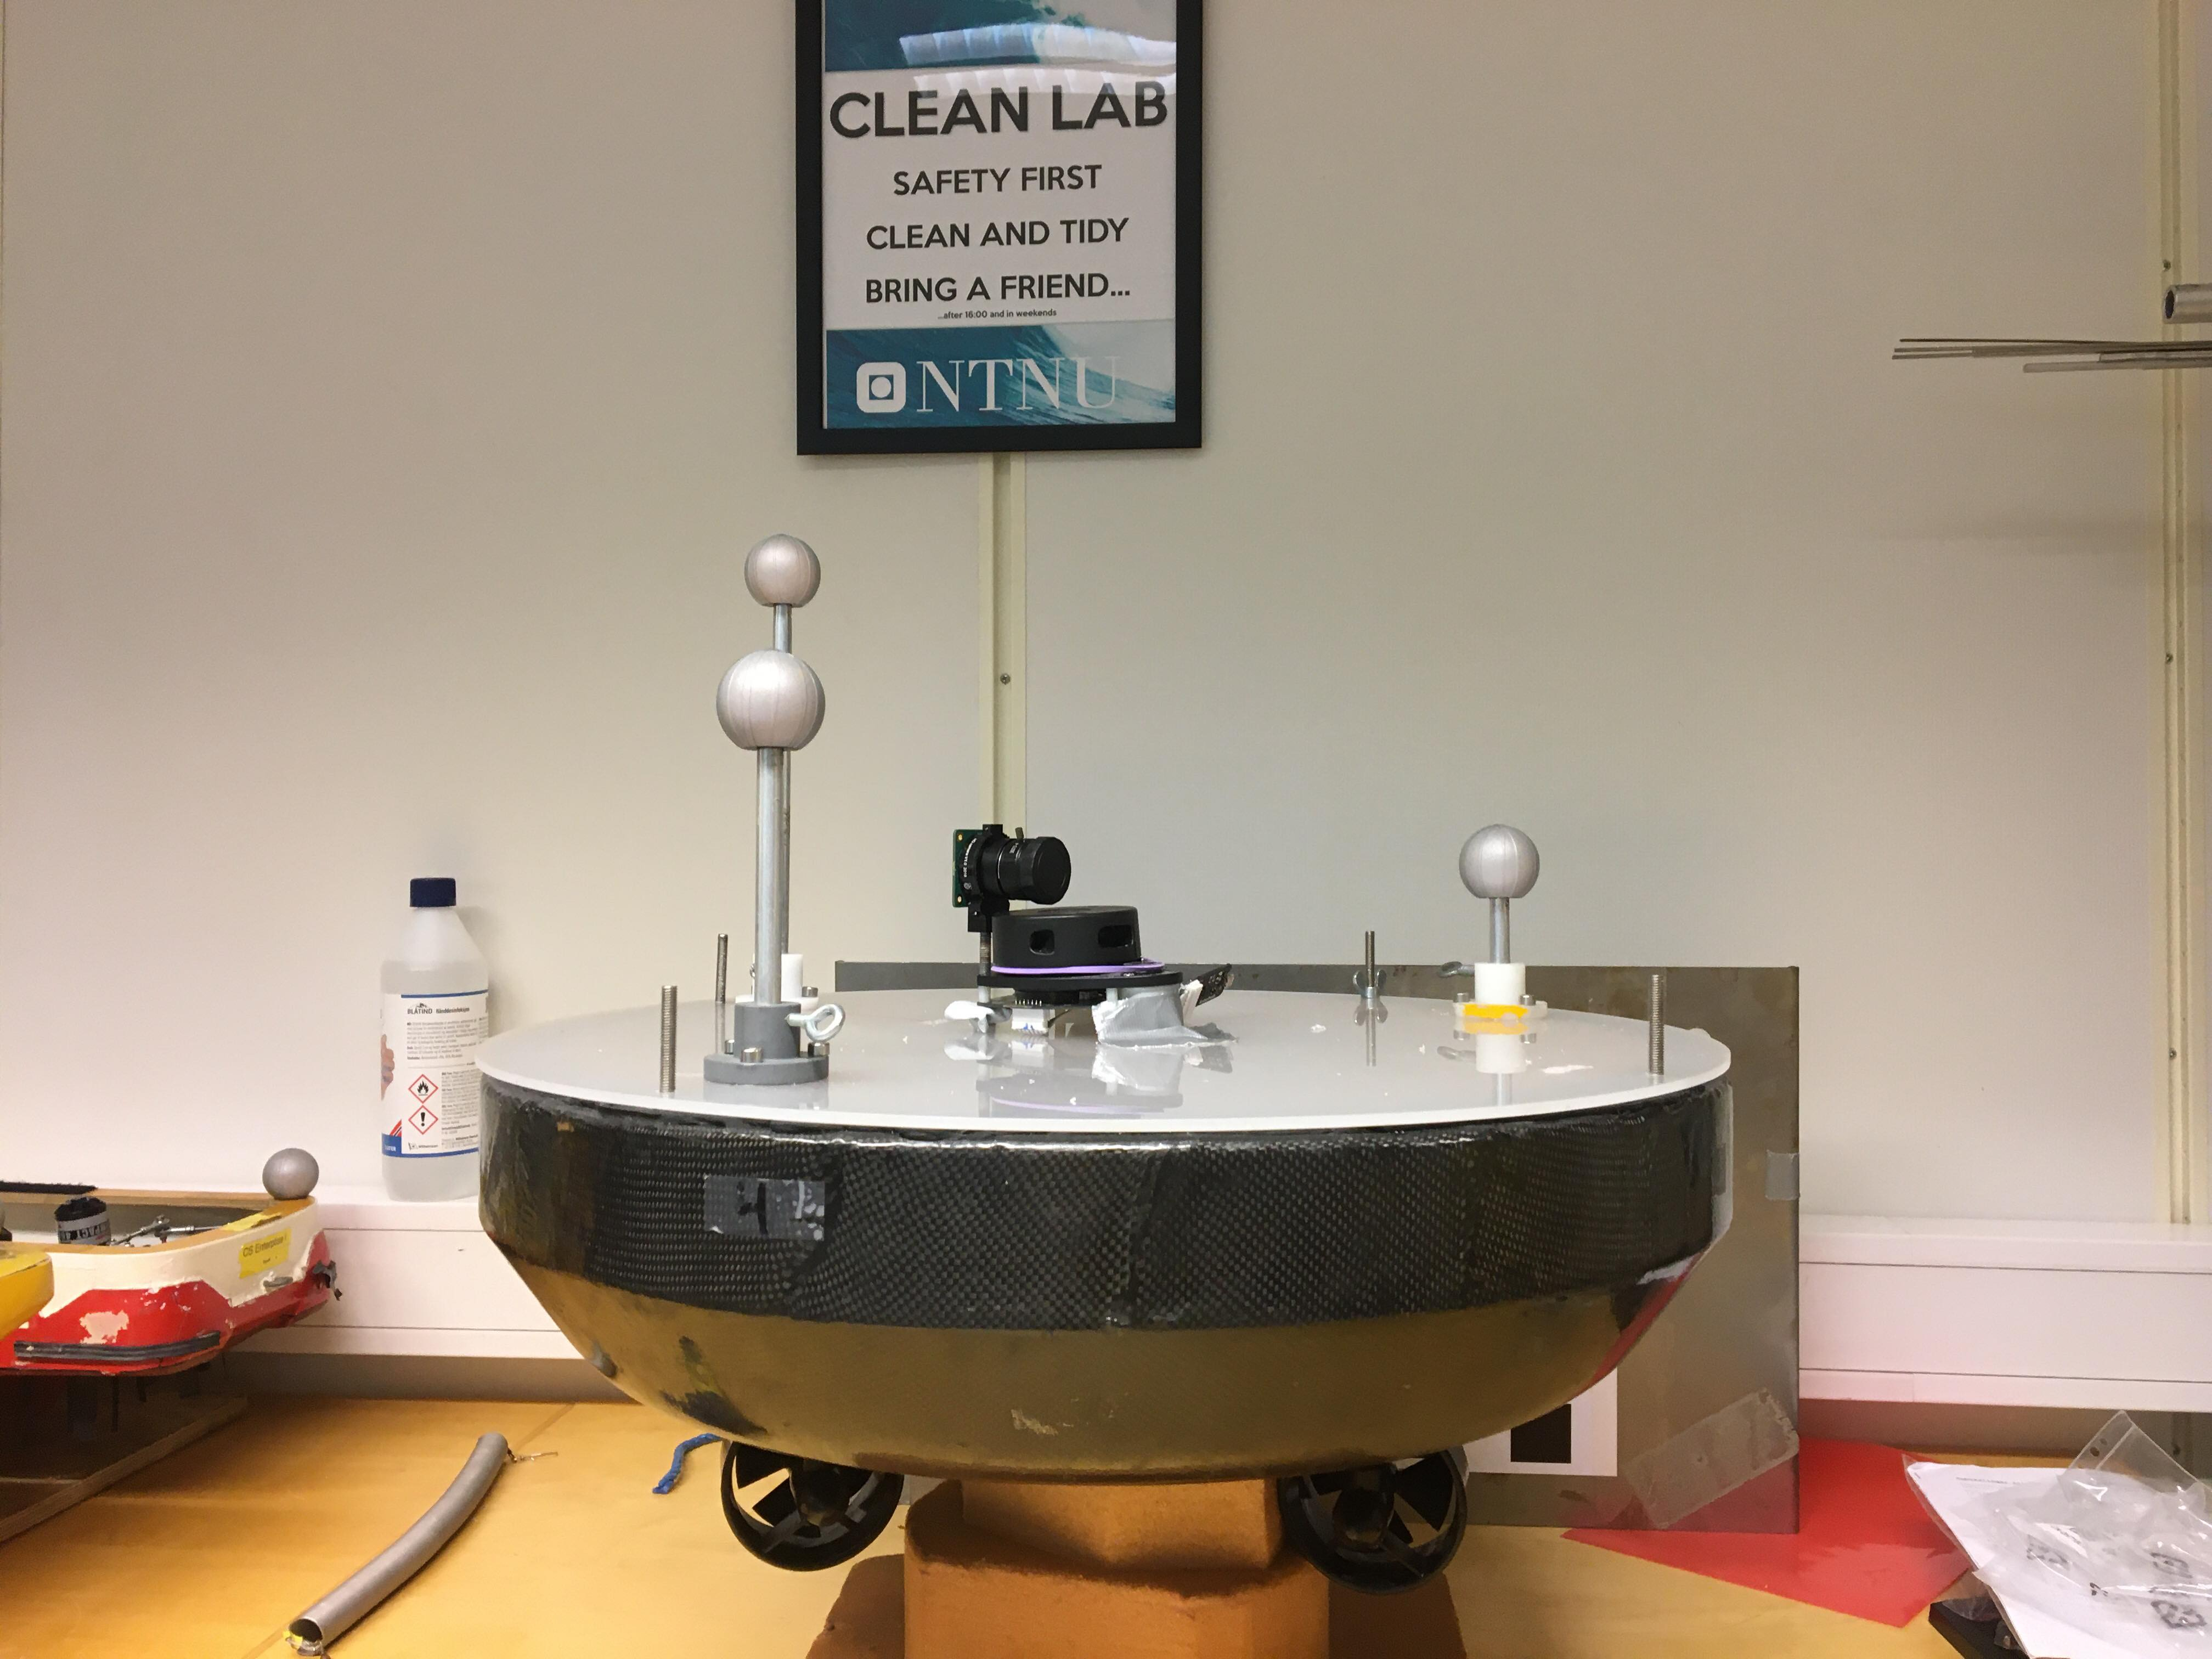
\includegraphics[width=0.8\textwidth]{Images/cssaucer.jpg}
    \caption{The CS Saucer with the latest module installed}
    \label{fig:suacer}
\end{figure}

A final upgrade to the Saucer was conducted as part of \citet{solheim-master}, harmonizing the system with the other vessels. 

\section{Literature}

The development of CSS is a product of much research from several theses, which contain complementary information on the theory applied to the system.

\subsection{Specialization projects and master theses}

\begin{itemize}
    \item Marine Cybernetics Vessel CS Saucer: - Design, construction and control - \citet{idland2015marine}
    \item Marine Inverted Pendulum - \citet{sharoni2016marine}
    \item Marine Autonomous Exploration using a Lidar - \citet{ueland}
    \item Sensor Fusion between camera and lidar for C/S Saucer - \citet{solheim}
    \item Integration between lidar- and camera-based situational awareness and control barrier functions for an autonomous surface vessel - \citet{solheim-master}
\end{itemize}

\section{Technical specification}

As part of the control system upgrade performed in this thesis, several new components were installed on the vessel. \cref{tab:techspec} provides a technical specification of the current state-of-the-art hardware utilized on the vessel. It also includes software utilized during operations. \cref{fig:signal-flow} illustrates the signal and power flow between each hardware component. For a more detailed review of the components, the reader is referred to either \citet{solheim} or \citet{ueland}. Components and software added as part of the control system upgrade are marked with a star ($\star$).

\begin{table}[H]
    \centering
    \begin{tabular*}{\linewidth}{ll}
    \toprule
    \multicolumn{2}{c}{\Large \textbf{Technical Specification}} \\
    \midrule
    \multicolumn{2}{l}{\large \textbf{Software}} \\
    \midrule
    Operating System & Ubuntu 20.04 LTS (Server version)$^\star$ \\
    ROS distrubution & Noetic$^\star$ \\ 
    \midrule
    \multicolumn{2}{l}{\large \textbf{Hardware}} \\
    \midrule
    \multicolumn{1}{l}{\textbf{Component}} &  \multicolumn{1}{l}{\textbf{Description}}\\
    \hline 
    Raspberry Pi 4b$^\star$ & Embedded computer for the vessel. Handles running \\ & ROS-nodes and communication between components \\ & in the system. \\ 
    &\textbf{Processor}: Quad-core Cortex-A72 @ 1.5 GHz.\\ 
    &\textbf{RAM}: 8 GB LPDDR4-3200 SDRAM\\ 
    &\textbf{Power}: 5V via USB-C \\
    \hline 
    Arduino Mega & Embedded circuit board responsible for transmitting \\ & appropriate PWM signals to each component.  \\ & Communicates with the RPi 4b via USB. \\ & Duty cycle between 4.3 and 9.4 \%. \\
    \hline
    Raspberry Pi HQ camera$^\star$ & Camera module \\
    & \textbf{Resolution}: 4056x3040 (12.3 Megapixels) \\
    & \textbf{Framerate}: 30 fps (at highest resolution) \\
    & \textbf{Sensor}: SONY IMX477 \\
    & \textbf{Lens}: 6mm wide angle \\
    \hline
    RPLidar A1 & Low cost $360^\circ$ 2D laser scanner with adjustable \\ & rotation speed. \\ 
    & \textbf{Effective range:} $\SI{12}{m}$ \\
    & \textbf{Sampling rate:}  $\SI{2000}{Hz}$ \\
    & \textbf{Angular resolution:} $\SI{1}{deg}$ \\
    & \textbf{Range accuracy:} $1\%<\SI{3}{m}$, $2\% \in [3, 5] \ m, 2.5\% > \SI{5}{m}$ \\
    \hline
    Torpedo 800 & Motor drive for the three azimuth thrusters. Can spin \\ & the propellers clockwise or counterclockwise. \\
    \hline
    Graupner Schuttel drive unit II & Servo driver to set azimuth angle. Can rotate on the \\ & interval $[-114^\circ, 114^\circ]$. \\
     \hline
    Traxxas LiPo & Three cell, $\SI{11.1}{V}$ lithium polymer battery. Powers \\ 
    & all devices on the vessel. At full charge, either $\SI{640}{mAh}$ \\ & or $\SI{500}{mAh}$, depending on the battery used, it can \\ & power the system for several hours. \\
    \bottomrule
    \end{tabular*}
    \caption{Technical specification for the CSS}
    \label{tab:techspec}
\end{table}

A second computer, referred to as the operator computer, is used together with the embedded computer on the CSS. The primary purpose of the computers is to run the computationally expensive visual detection and fusion nodes. Ideally, the computer should have a GPU to power the CNN, but since the system is designed with low computational availability in mind, a powerful CPU suffices. Therefore, for most of this thesis, a Dell laptop equipped with an 8-core Intel i5 vPro processor was utilized. Like RPi, the computer ran Ubuntu 20.04 LTS and ROS Noetic. 


\begin{figure}[H]
    \centering
    \begin{tikzpicture}
        
        \draw (0, 0) circle(5);
        \draw (0, 3.2) circle(0.8) node[text=black, every text node part/.style={align=center, font=\tiny}] (Motor1) {Motor and \\ Servo 1};
        \draw (2.8, -1.6) circle(0.8) node[text=black, every text node part/.style={align=center, font=\tiny}] (Motor3) {Motor and \\ Servo 3};
        \draw (-2.8, -1.6) circle(0.8) node[text=black, every text node part/.style={align=center,font=\tiny}] (Motor2) { Motor and \\ Servo 2};
        \node at (0, 0.5) [rectangle, draw,  text=black, every text node part/.style={align=center,font=\tiny}] (RPi) {Raspberry \\ Pi 4b};
        \node at (0, 1.5) [rectangle, draw, text=black, every text node part/.style={align=center,font=\tiny}] (Arduino) {Arduino};
        \node at (0, -0.5) [rectangle, draw, text=black, every text node part/.style={align=center,font=\tiny}] (Battery) {11.1V LiPo \\ Battery};
        \node at (1.65, 0.75) [rectangle, draw, , text=black, every text node part/.style={align=center,font=\tiny}] (Lidar) {Lidar};
        \node at (2, 0.25) [rectangle, draw, , text=black, every text node part/.style={align=center,font=\tiny}] (Camera) {HQ Camera};
        \node at (-9, -1) [rectangle,  minimum width = 3cm, draw, text=black, every text node part/.style={align=center,font=\tiny}] (Computer) {Remote \\ Computer};
        \node at (-9, 0) [rectangle, minimum width = 3cm, draw, text=black, every text node part/.style={align=center,font=\tiny}] (Qualisys) {Qualisys Motion \\ Capture};
        
        
        \draw[line width=0.4mm] (RPi) -- (Battery);
        \draw[line width=0.4mm] (Battery) -- (0, -1.6) -- (-2, -1.6);
        \draw[line width=0.4mm] (Battery) -- (0, -1.6) -- (2, -1.6);
        \draw[line width=0.4mm] (-1.5, -1.6) -- (-1.5, 3.2) -- (-0.8, 3.2);
        \draw[color=orange!60, line width=0.4mm] (0, 2.4) -- (Arduino);
        \draw[color=orange!60, line width=0.4mm] (0, 2.1) -- (-1, 2.1) -- (-1, -1.6);
        \draw[color=orange!60, dashed, line width=0.4mm] (-2, -1.6) -- (2, -1.6);
        \draw[line width=0.4mm] (RPi) -- (Lidar);
        \draw[dashed, color=red!60, line width=0.4mm] (RPi) -- (Lidar);
        \draw[line width=0.4mm] (RPi) -- (Camera);
        \draw[dashed, color=yellow!60, line width=0.4mm] (RPi) -- (Camera);
        \draw[line width=0.4mm] (RPi) -- (Arduino);
        \draw[dashed, color=red!60, line width=0.4mm] (RPi) -- (Arduino);
        \draw[dashed, color=blue!60, line width=0.4mm] (Computer) -- (RPi);
        \draw[dashed, color=blue!60, line width=0.4mm] (Qualisys) -- (RPi);
        \draw[dashed, color=blue!60, line width=0.4mm] (Qualisys) -- (Computer);
        \draw[blue, dashed, line width=0.4mm] (-8.75, 3) --node[above] {\tiny Wi-Fi} (-9.25, 3);
        \draw[yellow!60, line width=0.4mm] (-8.75, 3.5) --node[color=black, above] {\tiny Digital} (-9.25, 3.5);
        \draw[line width=0.4mm] (-8.75, 4) --node[color=black, above] {\tiny Power} (-9.25, 4);
        \draw[red!60, line width=0.4mm] (-8.75, 4.5) --node[color=black, above] {\tiny USB} (-9.25, 4.5);
         \draw[orange!60, line width=0.4mm] (-8.75, 2.5) --node[color=black, above] {\tiny PWM} (-9.25, 2.5);
    \end{tikzpicture}
    \caption{Signal and power flow between system components.}
    \label{fig:signal-flow}
\end{figure}


\section{Software}

\subsection{Robot Operating System}

The framework of the vessel's new control system is entirely based on the Robot Operating System (ROS). This section will, therefore, provide a brief introduction to ROS and its basic concepts. 

Introduced in 2007, ROS is an open-source project that provides tools, libraries, and conventions for robot applications. It functions as a meta-operating system (OS)  handling services you would expect from a conventional OS. These include hardware abstraction, message-passing between processes, and package management. 

A ROS process is represented as a node in a graph architecture. Nodes are connected to edges known as topics, through which they can pass messages to one another. They can also provide and make service calls to each other and send or retrieve data from a common parameter server known as the ROS-master. The ROS-master registers all active nodes to itself and establishes the peer-to-peer communication network of the nodes. Figure \ref{fig:ros-arch} illustrates the basic communication of a ROS-system.

\begin{figure}[H]
    \centering
    \begin{tikzpicture}
        \node at (-4.5,0) [rectangle, fill=cyan, text=black, draw, minimum width=2.5cm, minimum height = 1.5cm, every text node part/.style={align=center}] (Node1) {Node};
        \node at (4.5,0) [rectangle, fill=cyan,  text=black, draw, minimum width=2.5cm, minimum height = 1.5cm, every text node part/.style={align=center}] (Node2) {Node};
        \node[cylinder, draw = cyan, text = black, cylinder uses custom fill, 
               cylinder body fill = cyan!40, cylinder end fill = cyan!40, aspect = 0.3, 
               shape border rotate = 90] (c) at (0,2) (Master) {ROS-master};
        \node[rectangle, fill=gray, text=white, draw,  minimum height = 1.5cm,  minimum width = 1.5cm] at (0, -2) (Topic) {Topic};       
        \draw[dotted] (Node1) -- (Node2);
        \draw (0, 0) node[above]{\small Service invocation};
        \draw[-latex] (Node1) -- (-4.5, 2) -- (Master);
        \draw[-latex] (Node2) -- (4.5, 2) -- (Master);
        \draw[-latex] (Node1) -- (-4.5, -2) node[below, xshift=1cm] {\tiny Publishing} -- (Topic);
        \draw[-latex] (Topic) -- (4.5, -2) node[below, xshift=-1cm] {\tiny Subscribing} -- (Node2);
    \end{tikzpicture}
    \caption{Basic ROS concept}
    \label{fig:ros-arch}
\end{figure}

This decentralized architecture is the main strength of ROS, as it allows nodes to be run on separate, networked hardware. As each node process is isolated and messages passed between standardized, the implementation language of the node is also irrelevant. Effectively this means that one can run one or more nodes written in C++ in conjunction with nodes written in, for example, Python. This ties in with the last strength, the ROS ecosystem. ROS offers many easy and accessible software for robots as an open-source project, making integrating sensors a simple task. Most hardware comes with ROS support from the manufacturer or a third-party individual. As mentioned before, the software language is irrelevant, so one can easily download a C++ ROS driver and run it with a primarily Python-based system.

\subsection{ROS architecture}

Figure \ref{fig:ros-flow} illustrates the different node processes and message flow in the proposed ROS vessel control system from \citet{solheim-master}. Nodes are depicted as circles, with orange and red being sensor-related, blue being control system modules, and blue-grey being hardware nodes. \textit{Topics} are rectangles connected to nodes. If an arrow points from a node to the topic, the node is publishing to the relevant topic. Accordingly, arrows pointing to nodes from topics mean that the node subscribes to the given topic. The \textit{gain server} is a parameter-server that receives control- and observer gains from the operator, allowing the user to tune the system during operation.   

\begin{figure}[H]
    \centering
    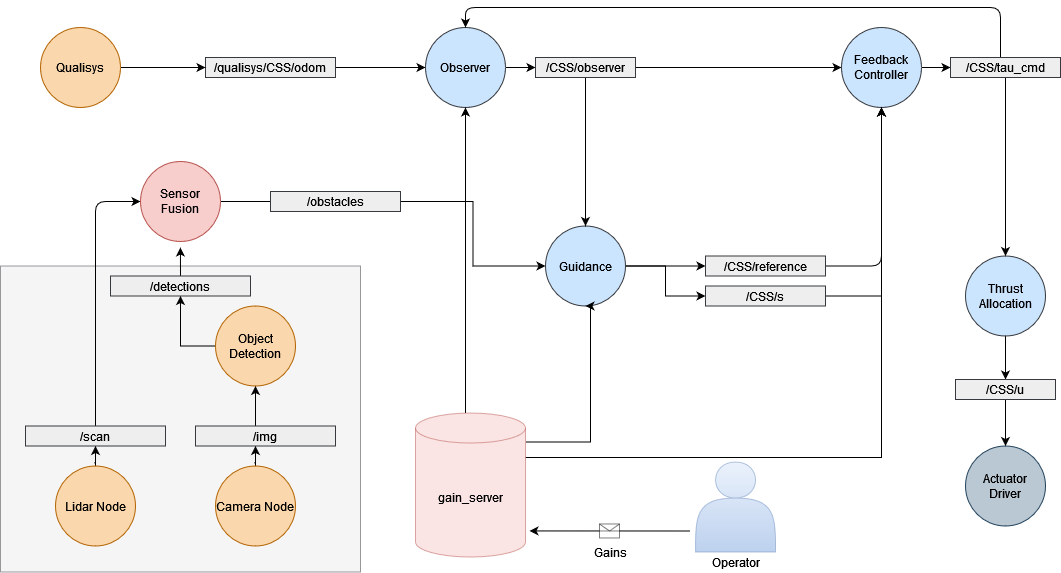
\includegraphics[width=\textwidth]{Images/ROS-topology(3).png}
    \caption{ROS-architecture of the CS Saucer.}
    \label{fig:ros-flow}
\end{figure}

\section{Vessel model}

\label{sec:modeling}

A mathematical model describing vessel dynamics is desirable in designing a control system and performing simulations. Starting from the equation of motion for a vessel at sea \citep{fossen_2021}, one can derive the necessary equations for the control model 

\begin{equation}
    \mathbf{M}_{RB}\dot{\boldsymbol{\nu}} + \mathbf{C}_{RB}\boldsymbol{\nu} + \mathbf{M}_A\dot{\boldsymbol{\nu}}_r + \mathbf{C}_A(\boldsymbol{\nu}_r)\boldsymbol{\nu}_r + \mathbf{D}(\nu_r)\nu_r + \mathbf{D}\boldsymbol{\nu}_r + \mathbf{g}(\boldsymbol{\eta}) = \tau_{ext},
\end{equation}

where:

\begin{itemize}
    \item $ \boldsymbol{\nu} = \big[ u \ v  \ r \big]^{\top}$ is the body-fixed velocities in surge, sway and yaw.
    \item $\boldsymbol{\nu}_r$ is the body-fixed velocities relative to local current in surge, sway and yaw
    \item $\mathbf{M}_{RB}$ and $\mathbf{M}_A$ is the vessel inertia matrix for mass and added mass
    \item $\mathbf{C}_{RB}$ and $\mathbf{C}_A(\nu_r)$ is the vessel Coriolis matrix for rigid body and added mass respectively. 
    \item $\mathbf{D}(\nu_r)$ is the nonlinear damping matrix
    \item $\mathbf{D}$ is the linear damping matrix
    \item $\mathbf{g}(\eta)$ is the hydro-static restoring matrix
    \item $\boldsymbol{\tau}_{ext} = \big[ X \ Y  \ N \big]^{\top}$ is the external forces acting in surge, sway and yaw
\end{itemize}

A model derivation was conducted by \citet{ueland} for his master thesis, which will be reused in this project. The following assumptions were made for the model: 

\begin{enumerate}
    \item Zero current in the MC-lab, $\nu_r = \nu$.
    \item The CSS is self-stabilizing by hydrostatic forces in heave, roll, and pitch. The rotations are considered small, so movements in surge, sway, and yaw are not affected by the configuration in pitch and roll. 
    \item No  hydrostatic restoring forces in surge, sway and yaw, $\mathbf{g}(\eta) = 0$.
    \item Constant frequencies, meaning that damping and added mass are also considered constant.
    \item The hull of the CSS is assumed to be completely symmetric.
\end{enumerate}

The resulting control design model is equivalent to the simplified model presented by \citet{fossen_2021}, which is a good representation of a 3DOF marine craft not affected by environmental forces, that is,

\begin{align*}
    \mathbf{\dot{\eta}} &= \mathbf{R(\psi)}\mathbf{\nu} \\
    \mathbf{M}\mathbf{\dot{\nu}} + (\mathbf{C} + \mathbf{D} + \mathbf{D}(\mathbf{\nu}))\nu &= \mathbf{\tau},
\end{align*}

where:

\begin{itemize}
    \item The inertia matrix $\mathbf{M}$
    \begin{equation}
    \mathbf{M} = \begin{bmatrix}9.51 & 0 & 0 \\ 0 & 9.51 & 0 \\ 0 & 0 & 0.116 \end{bmatrix}
    \end{equation}
    \item The Coriolis matrix $\mathbf{C}$
        \begin{equation}
    \mathbf{C} = \begin{bmatrix}0 & -9.51r & 0 \\  9.51r & 0 & 0  \\ 0 & 0 & 0 \end{bmatrix}
    \end{equation}
    \item The linear damping matrix $\mathbf{D}$
   \begin{equation}
    \mathbf{D} =  \begin{bmatrix}1.96 & 0 & 0 \\ 0 & 1.96 & 0 \\ 0 & 0 & 0.168 \end{bmatrix}
    \end{equation}
    \item The non-linear damping matrix $\mathbf{D(\nu)}$
    \begin{equation}
    \mathbf{D(\boldsymbol{\nu})} =  \begin{bmatrix}7.095|u| & 0 & 0 \\ 0 & 7.095|v| & 0 \\ 0 & 0 & 7.095|r| \end{bmatrix}
    \end{equation}
    \item The rotation matrix $R(\psi)$ 
    \begin{equation}
        \mathbf{R}(\psi) = \begin{bmatrix}\cos({\psi}) & -\sin{(\psi)} & 0 \\
        \sin{(\psi)} & \cos{(\psi)} & 0 \\ 0 & 0 & 1\end{bmatrix}
    \end{equation}
\end{itemize}

\section{Sensor integration}

A new top module was issued for the CSS as part of \citet{solheim-master} On top of it, two sensors were integrated along with tracking markers for the Qualisys motion capture system present in the MC-lab. The Qualisys system acts as a GPS for the vessel, providing the control system with measurements of the vessel's position and orientation. The markers are mounted on slender rods of varying heights along the circumference of the module. Then, the lidar is mounted in the center, directly above the CO of the CSS. The sensor is oriented so the $x_l$ and $y_l$ axis of the lidar align with the surge and sway directions, respectively. While the lidar provides a 360-degree scan, the interval of  $[-90^\circ, 90^\circ]$ is most interesting. Thus markers are mounted to cause as little interference as possible and still provide an accurate estimation of the vessel states. The same constraints apply to the placement of the camera. It requires an unobstructed view but can not interfere with the lidar in the critical area. Therefore it is mounted on a slender rod right behind the lidar with enough clearance to the lidar that it sees the environment clearly. The camera is tightly connected to the vessel heading, always pointing in the direction that is considered forward. Accordingly, it is mounted so that the $z_c$- and $x_c$-axis align with the surge and sway directions of the CSS.

\begin{figure}[ht]
     \centering
     \begin{subfigure}[b]{0.25\textwidth}
        \centering
        \begin{tikzpicture}
        \begin{scope}[scale=0.8]
        % place nodes
        \coordinate (a) at (0,0.5);% Change 1.5 to change the shape of the droplet
        \draw[semitransparent] (0,0) circle[radius=3cm]; % test of the radius size
        \draw[-latex] (0,0) -- (4, 0) node[below]{$\mathbf{Y}$};
        \draw[-latex] (0,0) -- (0, 4) node[left]{$\mathbf{X}$};
        \draw[fill=gray, semitransparent] (0,-2.45) circle[radius=5pt] node[left, xshift=-0.15cm] {\tiny Qualisys};;
        \draw[fill=gray, semitransparent] (2.45,0) circle[radius=5pt];
        \draw[fill=gray, semitransparent] (-2.05,1.2) circle[radius=5pt];
        \draw[-latex, dashed, red] (0,0) -- (2, 0) node[below]{$\mathbf{y_l}$};
        \draw[-latex, dashed, red] (0,0) -- (0, 2) node[left]{$\mathbf{x_l}$};
        \node [circle,draw, fill=gray, gray] (c) at (0,0) [minimum size=20pt] {$c$};
        \draw[gray, fill] (a) -- (tangent cs:node=c,point={(a)},solution=1) --
        (c.center) -- (tangent cs:node=c,point={(a)},solution=2) -- cycle;
        \draw[fill=black, semitransparent] (0, 0) circle [radius=8pt] node[left, xshift=-0.3cm] {\tiny LiDAR};
        \draw[-latex, dashed, blue] (0,-0.6) -- (2, -0.6) node[below]{$\mathbf{x_c}$};
        \draw[-latex, dashed, blue] (0,-0.6) -- (0, 1.4) node[left]{$\mathbf{z_c}$};
        \draw[fill=black] (-0.1, -0.5) rectangle(0.1, -0.7) node[left, yshift=-0.15cm, semitransparent] {\tiny Cam};
        \draw[fill=black] (0, -0.5) -- (-0.1, -0.45) -- (0.1, -0.45) -- (0, -0.5);
     \end{scope}
     \end{tikzpicture}
     \end{subfigure}
     \hfill
     \begin{subfigure}[b]{0.45\textwidth}
        \centering
        \begin{tikzpicture}
        \begin{scope}[scale=0.95]
        % place nodes
        \draw[semitransparent] (0, 0) rectangle (5.5, 0.1);
        \draw[fill=black, semitransparent] (0, 0) rectangle (5.5, -0.4);
        \draw[fill=black, semitransparent] (0, -0.4) -- (0.5, -0.8) -- (5, -0.8) -- (5.5, -0.4);
        \draw (2.725, 0.1) rectangle (2.775, 1);
        \draw[fill=gray] (2.75, 1.13) circle(4pt);
        \draw (4.1, 0.1) rectangle (4.15, 0.5);
        \draw[fill=gray] (4.125, 0.63) circle(4pt);
        \draw (0.45, 0.1) rectangle (0.5, 1.3);
        \draw[fill=gray] (0.475, 1.43) circle(4pt);
        \draw[fill=black] (2.45, 0.1) rectangle (2.5, 0.15);
        \draw[fill=black] (3, 0.1) rectangle (3.05, 0.15);
        \draw[fill=black] (2.40, 0.15) rectangle (3.1, 0.20);
        \draw[fill=black] (2.5, 0.15) rectangle (3, 0.35);
        \draw (2.25, 0.1) rectangle (2.30, 0.5);
        \draw[fill=black] (2.15, 0.5) rectangle (2.4, 0.7); 
        \draw[fill=black] (2.4, 0.6) -- (2.45, 0.7) -- (2.45, 0.5) -- (2.4, 0.6);
        \draw[-latex] (2.75, -0.5) -- (6, -0.5) node[above] {$\mathbf{X}$};
        \draw[-latex] (2.75, -0.5) -- (2.75, -2) node[left] {$\mathbf{Z}$};
        \draw[-latex, dashed, red] (2.75,0.25) -- (4, 0.25) node[below, xshift=-0.3]{$\mathbf{x_l}$};
        \draw[-latex, dashed, blue] (2.275, 0.6) -- (3.725, 0.6) node[above]{$\mathbf{z_c}$};
        \draw[-latex, dashed, blue] (2.275, 0.6) -- (2.275, -0.575) node[left]{$\mathbf{y_c}$};
        \end{scope}
    \end{tikzpicture}
     \end{subfigure}
        \caption{Sensor integration for the CS Saucer}
        \label{fig:sensor-suit}
\end{figure}

The open-source computer vision library OpenCV is utilized to establish an image stream between the camera and the object detection module. It provides a generic ROS camera driver that can be utilized with all Video4Linux (V4L2) compatible cameras and publishes the image stream to the ROS-topic \texttt{/cv\_camera/image\_raw}. In addition, Slamtec, the manufacturer of the RPLidar, provides a ROS driver for their hardware. The driver publishes the measured ranges to the topic \texttt{/scan}.
\chapter{Getting started with ROS}

This manual is intended to provide an introduction to the basic ROS procedures necessary to operate the CS Saucer in the Marine Cybernetics Library. It is intended for the use of future students at NTNU, whom to utilize the vessel for projects. The procedures presented in this manual are also generic enough that they apply to the other vessels of the cybership fleet. 

The author of this manual has spent countless hours troubleshooting software, and setting up an environment suitable for operation on the Raspberry Pi. The hope is that the provided procedures will shorten the time future students will have to use by providing better documentation. 

\section{Raspberry Pi Image}

Currently, all the vessels in the MC Lab  run a Raspberry Pi 4B as their embedded computer. The CSE1 and CSE1 run the same raspberry pi image with Raspbian Buster as the OS and Melodic as their ROS-distribution. 

For this thesis, the Raspbian Buster installation was insufficient, so a new image was created for this thesis. The main problem was that Raspbian Buster contained a fatal bug that prevents it from connecting to enterprise networks such as eduroam. Considering that much of the work is done on campus ground, and the Saucer required downloading a lot of software, a new operating system was installed for the Saucer. At the time of writing it runs Ubuntu 20.04 LTS Server edition, and ROS Noetic. Everything needed to run basic ros is installed, along with the computer vision library Open CV, Tensorflow and scipy as well. 

The student can choose which OS suits their needs and make an image of the memory card on either the CS Saucer or CS Enterprise for their own use. More information about this can be found \href{https://www.raspberrypi.com/software/}{here}. It is recommended to copy one of the memory cards rather than attempting a install from scratch. 


\section{Communicating with the Raspberry Pi}
\label{sec:commwithpi}
To communicate with the Raspberry Pi on the vessel, one needs to be connected to the 'MC lab' local network. After connecting to the network, open up a terminal and see if the vessel is also connected by running the command: 

\begin{lstlisting}[language=bash]
$ ping 192.168.0.108
\end{lstlisting}

Here the number-sequence is the IP of the Saucer. If  the RPi responds you can SSH onto it and run files via the terminal. Simply run the command

\begin{lstlisting}[language=bash]
$ ssh ubuntu@192.168.0.108
\end{lstlisting}

Most likely you will then be prompted for a password. All the RPi's have \textbf{\textit{marin33}} as the designated password. You are now ready to run commands on the raspberry pi remotely. 

\section{How to ROS: A step by step guide}

This section covers the basic ROS-commands you need to properly run scripts on either the RPi or your Ubuntu PC. 

\subsection{Sourcing ROS}

ROS-programs are generally run using command-line tools. Thus, we have to source our installation when we open a terminal. To source the installation run the command
\begin{lstlisting}[language=bash]
$ source /opt/ros/$ROS_DISTRIBUTION$/setup.bash
\end{lstlisting}

The ROS-distribution will either be called \textit{melodic} or \textit{noetic}, depending on which vessel you use. On the provided hardware ROS is sourced automatically via a bash-script every time you open the terminal, but if you are using your own computer you will have to do this for ROS commands to function.

\subsection{Creating a workspace}

Next, we need to create a designated workspace for our project. Navigate to the desired location on your computer (/documents, for example) and create a new folder for your project by running the following command

\begin{lstlisting}[language=bash,]
$ mkdir -p my_folder/src
\end{lstlisting}

This creates a folder with a sub-directory called \textit{src}. You can replace \textit{my\_folder} with any name you want, but \textit{src} must be kept the same. Standard ROS-convention is prefixing your workspace folder with \textit{ws}, e.g \textit{ws\_dplab}.

Next, navigate to the workspace folder, and run the command

\begin{lstlisting}[language=bash]
$ catkin_make
\end{lstlisting}

This will build your workspace environment with the proper ROS dependencies. After running this command, you should be left with a directory structure that looks like this: 

\dirtree{%
.1 my$\_$folder.
.2 build.
.2 devel.
.2 src.
}

You are now ready to run ROS-files. As you add more packages to your project, it is good to rebuild your project. This is done by running the \textit{catkin\_make} again.

\subsection{The src-directory}
\label{sec:src}
This is the folder you will be working the most in, and were you will be putting all your ROS-packages. Each of these packages contain its own \textit{src}-directory where the scripts you will be using are located. A typical project folder can look something like this: 

\dirtree{%
.1 my\_folder.
.2 build.
.2 devel.
.2 src.
.3 simulator.
.4 launch.
.4 src.
.5 CSS.py.
.3 feedback\_controller.
.4 launch.
.4 src.
.5 ctrl\_joy.py.
}

\subsection{Running ROS nodes}
\label{sec:run-nodes}
After your code is written it is time two activate your ROS-nodes.

\subsubsection{The ROS-master}

First we need to make sure the ROS-master is running. On the raspberry-pi, this should be activated automatically. If you are running on the Ubuntu-computer you will have to enable it manually. Open a new command-line window and run the command: 

\begin{lstlisting}[language=bash]
$ roscore
\end{lstlisting}

Now the ROS-master is running, and you can start activating nodes.

If you are running nodes on separate computers, you need to make sure the computer not running the master knows were to find it. This is done by exporting the url for the ROS master. Before running any nodes, use the following command: 

\begin{lstlisting}[language=bash]
 $ export ROS_MASTER_URI=http://192.168.0.108:11311
\end{lstlisting}

 It is also smart to export the ROS\_IP. This tells the master were the signals are coming from. You can determine your IP by running the command \texttt{ifconfig} and then 
 
 \begin{lstlisting}[language=bash]
 $ export ROS_IP=YOUR IP
\end{lstlisting}



\subsubsection{Activating nodes}
In a separate command-line window, navigate to your project folder. Then source the setup.bash file in \textit{devel}. 

\begin{lstlisting}[language=bash]
$ source devel/setup.bash
\end{lstlisting}

To activate a node, we first need to make sure that the script is executable. To make a file executable, navigate to the relevant directory and run the following command: 

\begin{lstlisting}[language=bash]
  $ chmod +x <node-script>.py
\end{lstlisting}

If the script has become executable, the file-name should be green the next time you run \textbf{ls} inside the directory. Then, to activate a node run navigate to the base directory of your workspace and run 

\begin{lstlisting}[language=bash]
$ rosrun <package-name> <node-script>.py
\end{lstlisting}

where $<$package-name$>$ is the name of the package you want to run, e.g "controller", and the $<$node-script$>$.py is the python script that initializes the rosnode, e.g "ctrl\textunderscore joy.py".

\subsection{Launch files}

As a project progresses, more and more nodes are typically added. The process of activating nodes can therefore become more tedious as the complexity increases. To avoid having to open new command-line windows for every node, we can instead use \textit{launch-files} to activate multiple nodes simultaneously. A launch file is easy to create, and is placed in the \textit{launch} directory of a package, as illustrated in the directory-tree in section \ref{sec:src}.

\begin{listing}[h]
\inputminted{octave}{Code/example.launch}
\caption{Example of a launch-file}
\label{listing:launch}
\end{listing}

Listing \ref{listing:launch} shows the basic setup of a launch file. This example launches four separate nodes, the simulator, an observer, the guidance module and the controller module. 

To run a launch file we use the following command: 

\begin{lstlisting}[language=bash]
$ roslaunch <package_name> my_launchfile.launch  
\end{lstlisting} 

Replace package\textunderscore name with the name of the package you placed your launch file in. All launch files have the .launch ending (e.g DP-system.launch) . 

\subsection{Topics}

When nodes are activated, they will start to either \textit{publish} or \textit{subscribe} to \textit{topics}. Topics are named buses over which nodes exchange messages. We can any topics that are being published/subscribed to in a ROS-system by using the command: 

\begin{lstlisting}[language=bash]
$ rostopic list 
\end{lstlisting} 

This will display all the active topics in a list in your terminal. In a DP-system we might, for example, have a thrust allocation algorithm that publishes actuator commands $u$ to a topic that a the driver of the thrusters subscribes too. This topic is called something like \textbf{CSS/u}. If we wish to display the signals from this topic in real time we can run the command

\begin{lstlisting}[language=bash]
$ rostopic echo CSEI/u
\end{lstlisting}
This will print every message that is sent to the given topic, and can be a useful tool when debugging.

\subsection{Storing data}

It is desirable to store the message-signals in the system in some format so that we can later analyze and plot the data. ROS provides its own tools and file-format for this, called a \textit{bag} file. After we have launched some nodes we run the command 
\begin{lstlisting}[language=bash]
$ rosbag record <topic>
\end{lstlisting}

$<$Topic$>$ is replaced with the names of the topics we wish to save. Multiple topics can be recorded at the same time, in the same bag file. You just have to list the topic names with a space. If i for example wanted to record the commanded force signal from our control law and the resulting actuator commands form the thrust allication i would use 

\begin{lstlisting}[language=bash]
$ rosbag record CSS/u CSS/tau
\end{lstlisting}

When you have collected sufficient data, simply use CTRL+C to abort the operation. The data will be saved in a bag-file in your workspace.

\subsection{Other usefull ROS-commands}
\begin{lstlisting}[language=bash]
$ rosnode list
\end{lstlisting}
Shows a list of all active ROS-nodes

\chapter{Control system manual}

\section{System requirements}

The following is a list of all software required to run the control system implemented in this thesis. The are split into to parts, general software, python libraries and ROS-packages.

\begin{table}[H]
    \centering
    \begin{tabular*}{\linewidth}{ll}
    \toprule
    \multicolumn{2}{c}{\Large \textbf{\quad \quad \quad Requirements}} \\
    \midrule
    \multicolumn{2}{l}{\large \textbf{General}} \\
    \midrule
    Operating System & Ubuntu 20.04 LTS (Server version) \\
    ROS distrubution & Noetic \\ 
    Python &  3.8+ \\
    GCC & 8+ \\
    OpenCV & \\
    \midrule
    \multicolumn{2}{l}{\large \textbf{Python libraries}} \\
    \midrule
    Numpy 1.19.5+ & \\
    tensorflow & \\
    openCV & \\
    scipy & \\
    qp\_solvers & \\
    cvxopt & \\
    ds4drv & \\
    \midrule
    \multicolumn{2}{l}{\large \textbf{Ros packages}} \\
    \midrule
    CV-camera & \\
    CV-bridge & \\
    rplidar & \\
    rosserial & \\
    ds4\_drivers & \\
    dynamic\_reconfigure & \\
    \bottomrule
    \end{tabular*}
    \caption{Required software}
    \label{tab:requiredsoftware}
\end{table}

\section{Running the control system nodes}

This section will describe the procedure for running the available control system. First, one must SSH onto the raspberry pi as described in \cref{sec:commwithpi}. Den navigate to the workspace. It should be called \texttt{ws\_saucer}. Source the setup.bash file, and we are ready to start. 

\subsection{Dualshock 4 driver}
 
The system relies on the playstation ds4-driver, so we start by launching this node. Its package should be in the directory. To activate the driver, run the command

\begin{lstlisting}[language=bash]
$ roslaunch ds4_driver ds4_driver.launch use_standard_messages:=True
\end{lstlisting}

Running a roslaunch command will automatically start the ROS-master if you do not have one running. To connect the bluetooth controller, simply press the button on the middle. The controller should light blue when connected and an ouput should be printed in the terminal window. If the controller is not paired, you can follow this \underline{\href{https://ubuntu.com/core/docs/bluez/reference/pairing/outbound-pairing}{tutorial}}.


\subsection{Camera}
\label{sec:camera-driver}
Next up is the camera node. Open a new terminal. For this driver you do not have to be in the workspace. 

\begin{lstlisting}[language=bash]
$ rosrun cv_camera cv_camera_node
\end{lstlisting}

You should see an ouput that the calibration file was loaded if successfully activated. 

\subsection{Lidar}
\label{sec:lidar-driver}
To activate the lidar, open a new terminal and navigate to the workspace folder again. Then run the command

\begin{lstlisting}[language=bash]
$ roslaunch rplidar rplidar.launch 
\end{lstlisting}

Again, if successful you should see an output in the terminal. If it tells you the firmware is deprecated, just ignore the warning. 

\subsection{Arduino}

Finally, before we activate the motion control system we must enable one final node. This is the node on the Arduino that subscribes to the pwm signals. To enable it, run 

\begin{lstlisting}[language=bash]
$ rosrun rosserial_python serial_node.py _port=:dev/ttyACM0
\end{lstlisting}

Here the final argument specifies which usb port the arduino is connected to on the raspberry pi. It may vary, so to check run 

\begin{lstlisting}[language=bash]
$ ls /dev
\end{lstlisting}

to see which devices are connected. 

\subsection{Motion Control System}

Finally, we can activate the motion control system. In the workspace folder run 

\begin{lstlisting}[language=bash]
$ roslaunch feedback_controller collision_avoidance.launch
\end{lstlisting}

This should activate necessary nodes. The system defaults to manual control with the joystick controller, but can switch to automatic by pressing the triangle button on the ds4 controller. The guidance is activated by pressing square. Note that this should not be done unless the vessel is in the basin, and the object detection node is active. 

If one wishes to for example test one node, each package can be launched individually using the guidelines from \cref{sec:run-nodes}.

\subsection{Object detection}

On your operator computer, navigate to the workspace folder of your choice. Remember to export the ROS master url to establish communication between the nodes. To run the SA system use the following command

\begin{lstlisting}[language=bash]
$ rosrun objdetection detection_node
\end{lstlisting}

This will open a window with video-feed from the saucer on your operator computer. 


\section{Dynamic Reconfigure}

To make tuning your controller and observer more effective, tools for dynamic tuning are provided in the form of the ROS-package gain\_server. This allows you to change the gains in real time, rather than having to hard-code the gains and then stopping and starting your system every time you want to change them. To activate the node, and GUI use the following steps

Run the node use the command:
\begin{lstlisting}[language=bash]
$ rosrun gain_server server.py
\end{lstlisting}
\textbf{NOTE!} If you use the dynamic tuning, you should always activate this node \textbf{first} or you may experience errors. This is because the subscriberss in guidance, observer and controller nodes will expect values to be there when they are not. When the node is activated, the initial gains should be printed to your terminal. If you use the collision\_avoidance.launch file the gain\_server node will be started as part of this, and you can disregard the first step. 
    
 In another terminal, activate the GUI: 
\begin{lstlisting}[language=bash]
$ rosrun rqt_gui rqt_gui -s reconfigure
\end{lstlisting}
    
This should open a program that looks like this: 
    
\begin{figure}[H]
    \centering
    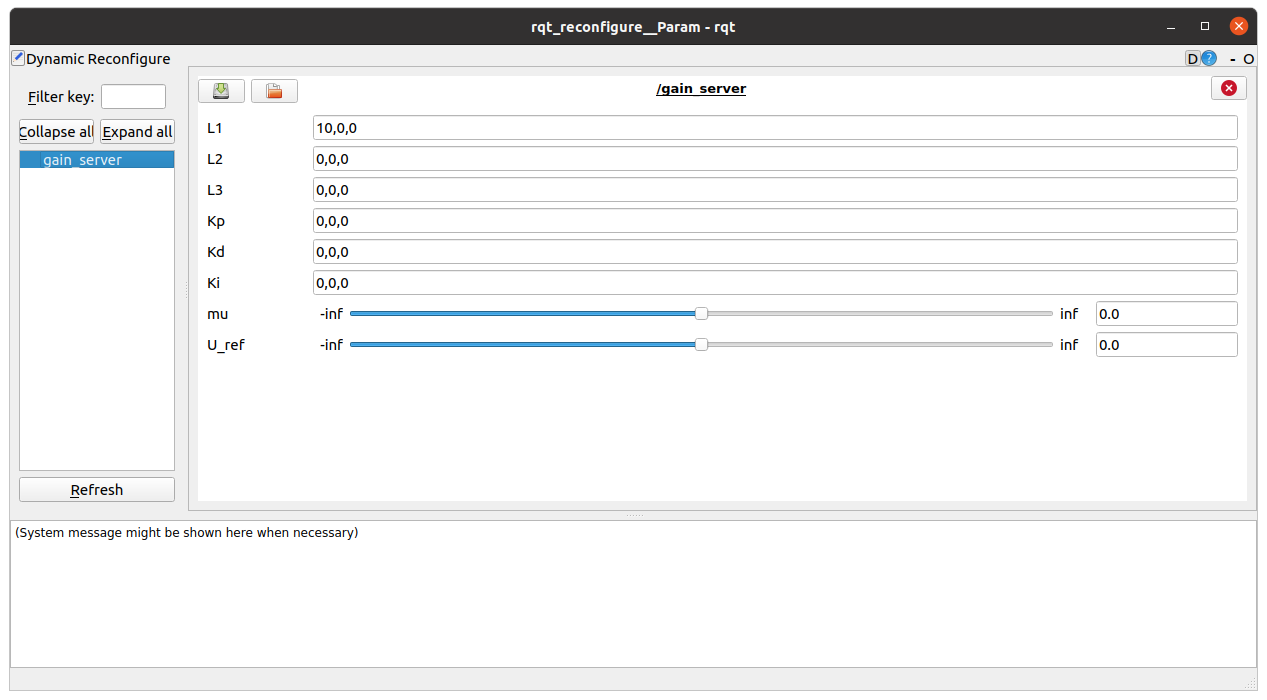
\includegraphics[width=\textwidth]{Images/dynamic-reconfigure.png}
    \caption{Tuning GUI}
    \label{fig:tuner}
\end{figure}
    
Each field or slider here corresponds to a gain in either the observer or controller. Not all the variables are relevant either. The last to are single float values, while the first six are meant to represent the elements on the diagonal of a $3\times3$-matrix. Change these to tune you controller. 

\chapter{Calibration Procedures}

This manual is meant to walk the user through calibrating the situational awareness system of the CS Saucer. It encompasses the camera calibration and then the lidar and camera calibration procedures. 

\section{Camera calibration}

First, make sure that the camera is correctly mounted, and that the ribbon cable is connected to the Raspberry Pi. For this calibration, you will need a checkerboard pattern. You can find some in the MC Lab, or print out your own on an A3 paper. It is recommended that you laminate the checkerboard so you can use it multiple times. The pattern used in this thesis was 9x7 squares with the length of 40 mm. The exact number and size is arbitrary as long as it is specified to the software. Place the Saucer somewhere high enough that you can move quite freely in the camera frame. 

SSH on to the Raspberry pi via your operator computer, and run the camera driver as outlined in \cref{sec:camera-driver}. Then in a separate terminal window on the operator computer (not the RPi!) run the following comand:

\begin{lstlisting}[language=bash]
$ rosrun camera_calibration cameracalibrator.py --size 8x6 --square 0.40 image:=/cv_camera/raw_image camera:=/cv_camera
\end{lstlisting}

Here --size is the argument for number of inner corners in the pattern and --square the length of the sides. If the node is successfully activated, you will be met with the following window: 

\begin{figure}[H]
    \centering
    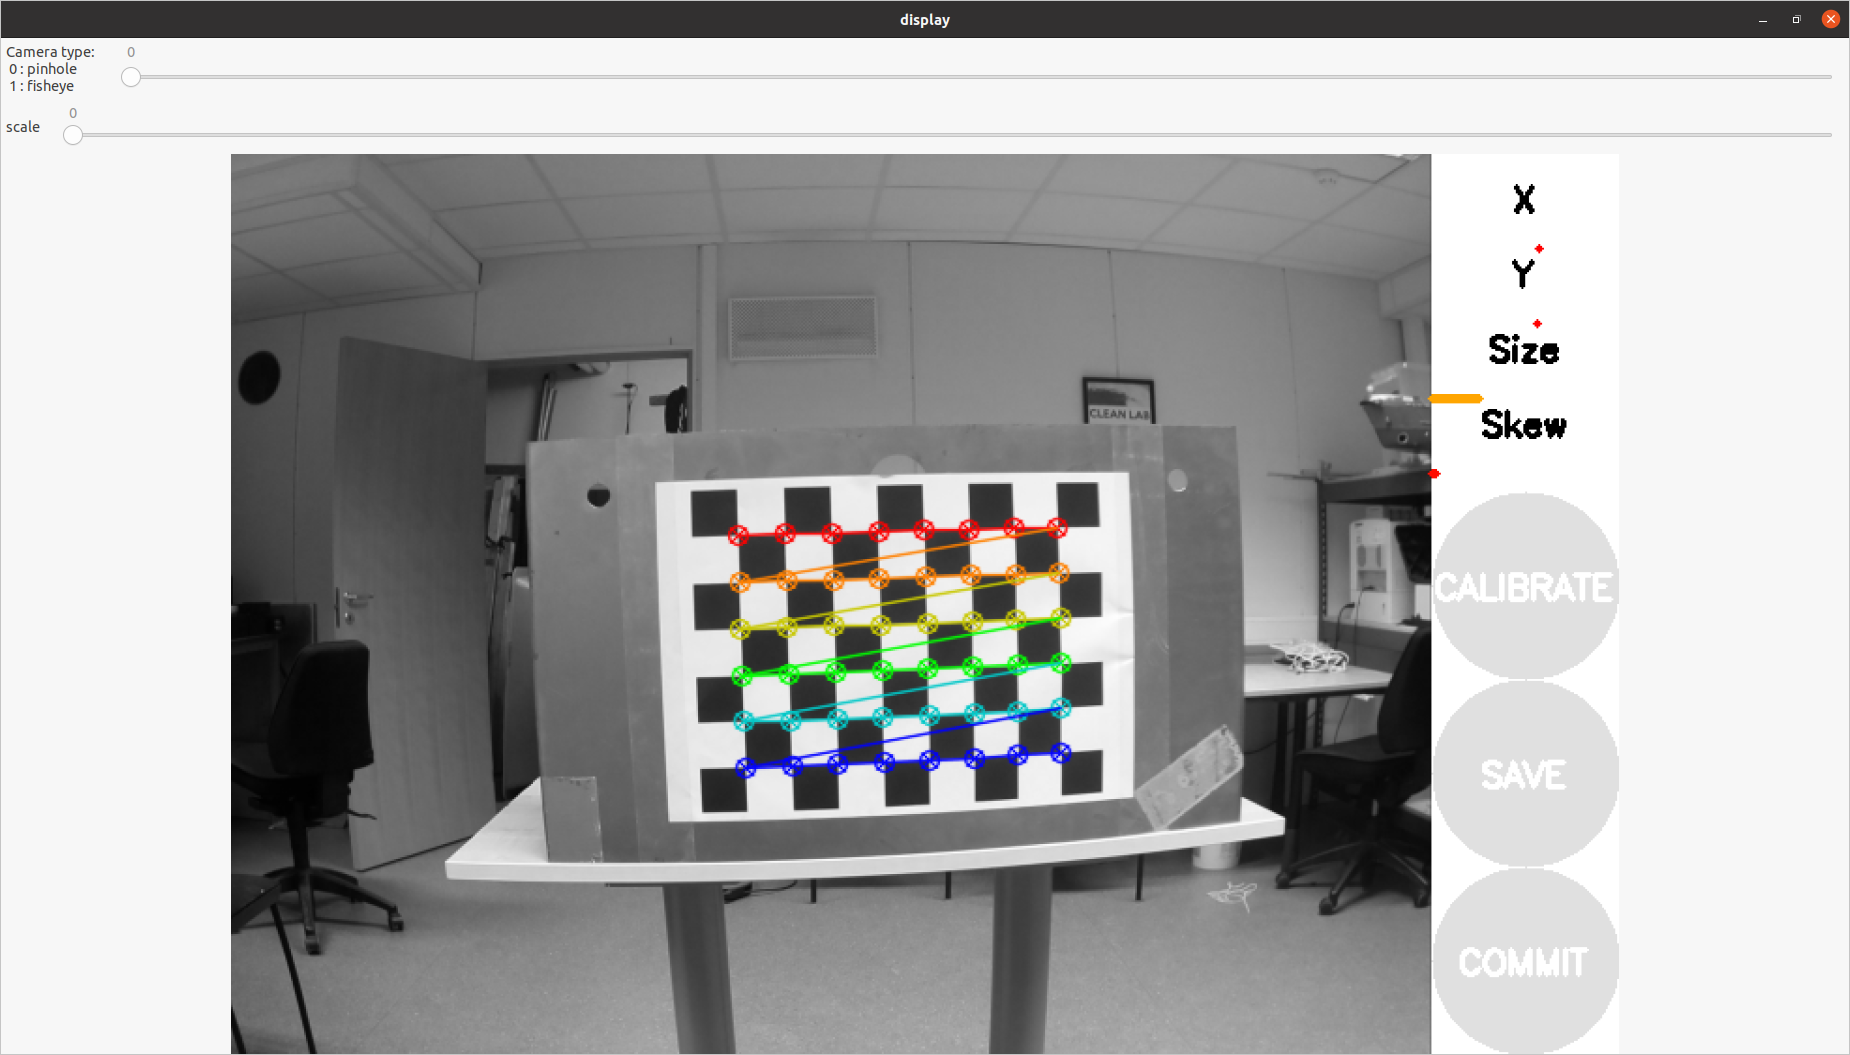
\includegraphics[width=\textwidth]{Images/camera-calibration.png}
    \caption{Calibration window}
    \label{fig:calibration-window}
\end{figure}

Move the checkerboard around in different orientations, at different distances in the camera frame. The program will grab data-samples as you go. When the bars on the right of \cref{fig:calibration-window} are full enough, the calibrate button will turn a darker shade of grey. This means that enough data has been collected to produce a calibration. You can keep going to produce a more accurate calibration. When you are finished, simply press the cailbrate button and the procedure will start. After it is over, the intrinsic parameters will be printed to the terminal window. To save these, press commit. This will make sure that the camera driver on the raspberry pi, always launches with these intrinsic parameters. You can also save the parameters to a file using the 'Save' button. Now you can exit the window. 

\section{Camera-Lidar calibration}

The software for the lidar-camera calibration is based on \cite{calibration-repo}. However, some changes have been made, so it is recommended that you use the files provided electronically with the thesis. Copy the calibration workspace over to your operator computer, and build it. Make sure you clean the files in the directory \textit{data}. In the directory calle \textit{config}, edit the config.yaml file to contain the intrinsic camera  parameters you obtained from the camera calibration.

Next you should identify the geometry you wish to use as your anchor points, and measure the height up to the lidar from the floor. Then, mark that height with tape on the corners inside the cameras point of view. 

Then you can SSH onto the RPi and start the lidar and camera according to \cref{sec:lidar-driver} and \cref{sec:camera-driver}. On the operator computer, in the calibration workspace, run the command 

\begin{lstlisting}[language=bash]
$ roslaunch camera_2d_lidar_calibration collect_camera_calibration_data.launch
\end{lstlisting}

This will print you camera parameters in the terminal and activate the program RViz, as seen in \cref{fig:yup}

\begin{figure}[H]
    \centering
    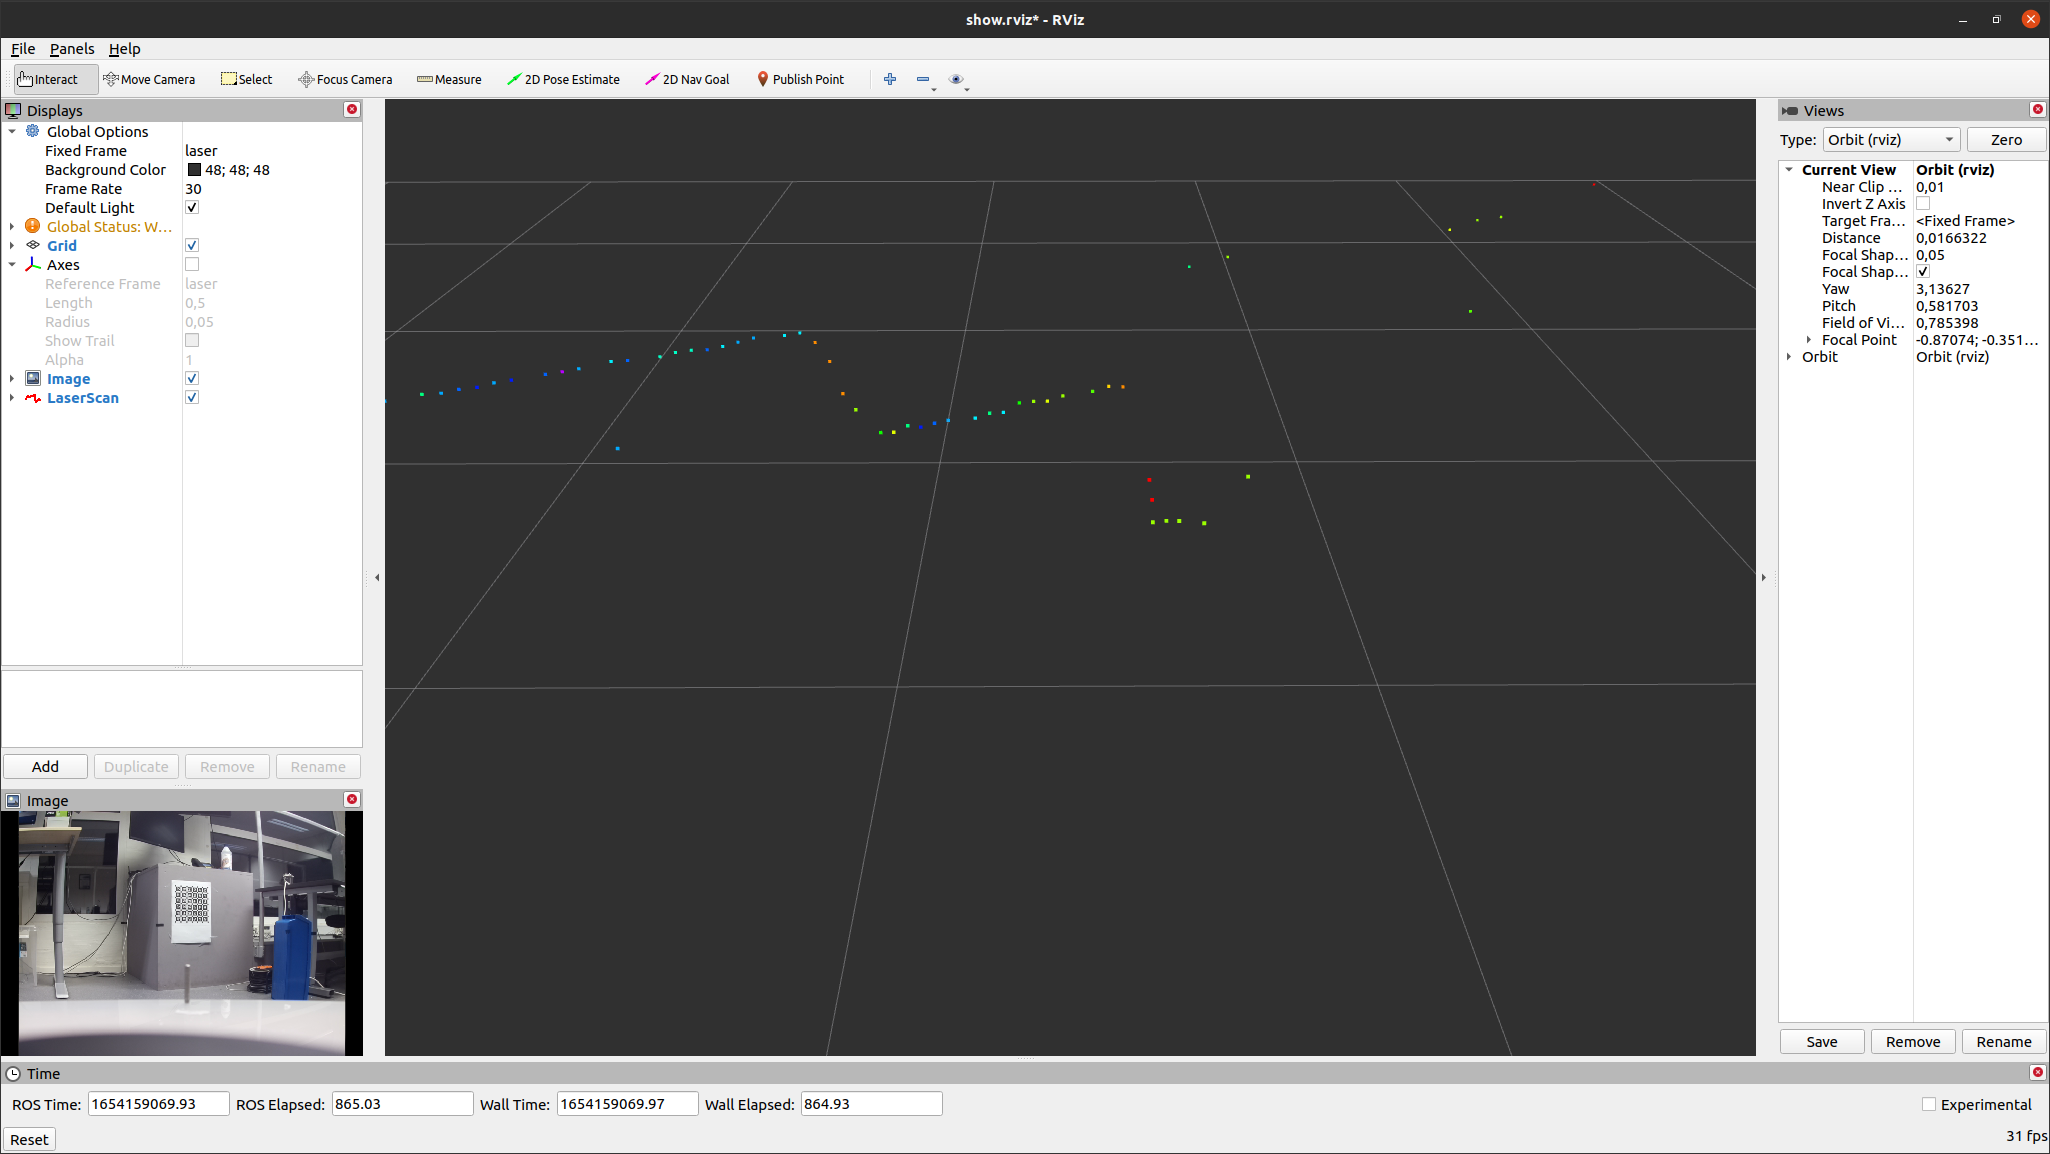
\includegraphics[width=\textwidth]{Images/actual-laz-cal.png}
    \caption{RViz window for calibration}
    \label{fig:yup}
\end{figure}

Then using the \textbf{2D Nav Goal} tool from the top bar, pick a point from the laser point cloud that corresponds to a corner. This will prompt the following window in \cref{fig:pixel-value}


\begin{figure}[H]
    \centering
    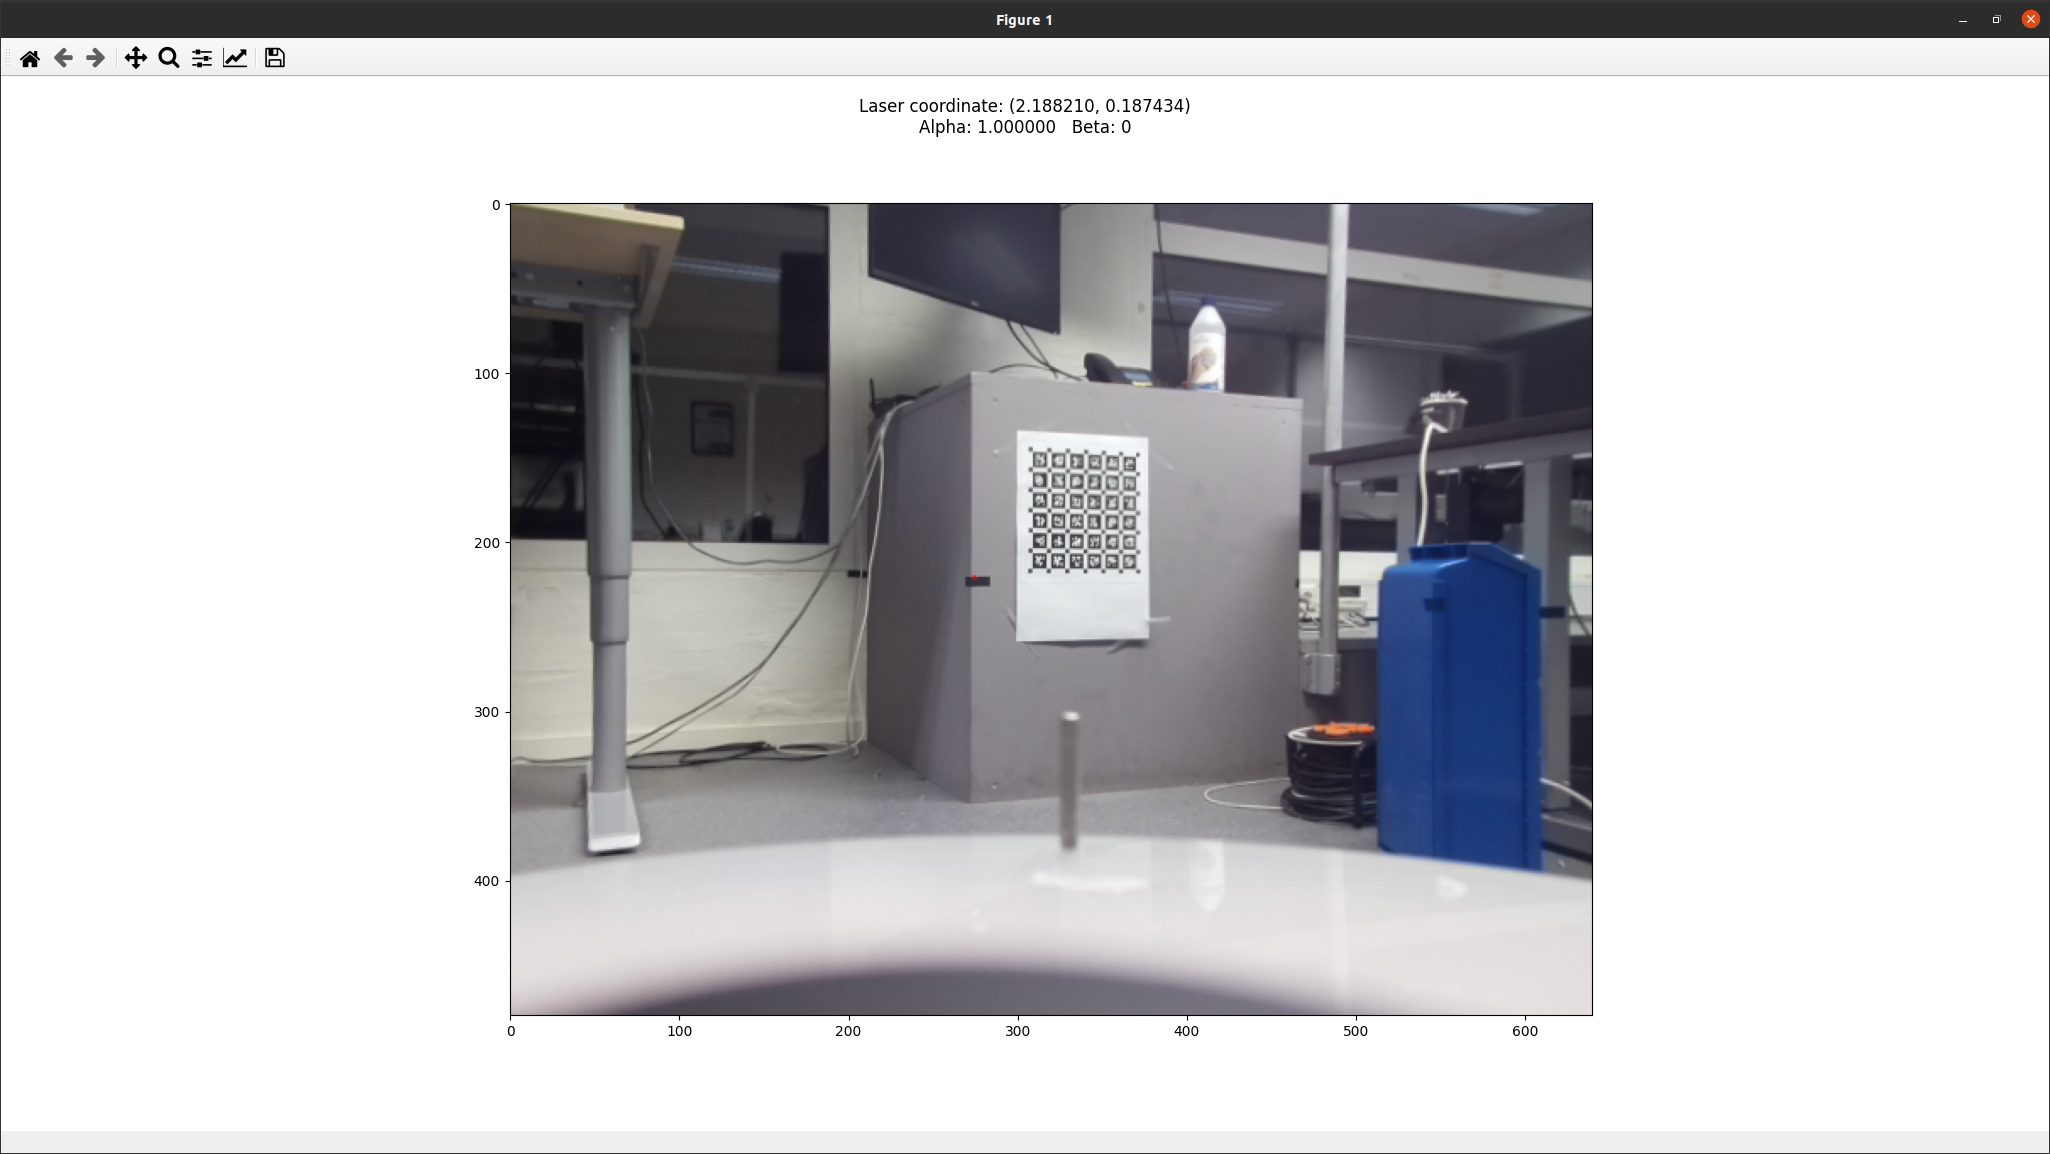
\includegraphics[width=\textwidth]{Images/choose-point.png}
    \caption{Choosing corresponding pixel value}
    \label{fig:pixel-value}
\end{figure}

Mark the area in the image that corresponds to the lidar point you chose. This is not an exact science, but try to be as accurate as you can. When satisfied with the point placement, press space and the window will close and the point be saved. Repeat the process several times for all the corners until you get enough data points. 10-20 should suffice, try to reduce the RMSE as much as possible. After you have enough data, close RViz and in the terminal run the second command

\begin{lstlisting}[language=bash]
$ roslaunch camera_2d_lidar_calibration calibration.launch
\end{lstlisting}

This will run the camera and lidar calibration procedure and spit out the rigid body transformation along with the root mean square error. You can check the translation with hand-measurements, if they are in the same ballpark the calibration is ok. You can now try to reproject the laser point onto the live image. This is done by running 

\begin{lstlisting}[language=bash]
$ roslaunch camera_2d_lidar_calibration reprojection.launch
\end{lstlisting}

Here you can see how the lidar points line up with the tape. 

\newpage
\printbibliography[heading = bibintoc, title = References] 

\end{document}


